\documentclass[11pt]{article}
	
	%%%%%%%%%%%%%%%%%%%%%%%%%%%%%%%%%%%%%%%%%%%%%%%%%%%%%%%%%%%%%%%%%%%%%%
	%\pdfminorversion=4
	% NOTE: To produce blinded version, replace "0" with "1" below.
	\newcommand{\blind}{0}
	
	%%%%%%% Margin specifications %%%%%%%%%%%%%%%%%%%
	% DON'T change margins - should be 1 inch all around.
\usepackage{geometry}
 \geometry{
 a4paper,
 total={170mm,257mm},
 left=18mm,
 top=18mm,
 }
    %%%%%%%%%%%%%%%%%%%%%%%%%%%%%%%%%%%%%%%%%%%%%%%%%%%%%%%%%%%%%%%%%%%%%%%%%
	
	%%%%% IISE Transactions package list %%%%%%%%%%%%%%%%%%%%%%%%%%%%%%%%%%%%%%
	\usepackage{amsmath}
	\usepackage{graphicx}
	\usepackage{enumerate}
	\usepackage{xcolor}
	\usepackage{xcolor}
	\usepackage{natbib} %comment out if you do not have the package
	\usepackage{url} % not crucial - just used below for the URL
	\usepackage[document]{ragged2e}
	\usepackage{hyperref}
	\usepackage{algpseudocode}
	

%% BibTeX settings
\usepackage{natbib}
\bibliographystyle{apalike}
%\bibliographystyle{unsrtnat}
\bibpunct{(}{)}{,}{a}{,}{,}


%% paragraph formatting
\renewcommand{\baselinestretch}{0.8}


% Defines columns for tables
\usepackage{array}
\newcolumntype{L}[1]{>{\raggedright\let\newline\\\arraybackslash\hspace{0pt}}m{#1}}
\newcolumntype{C}[1]{>{\centering\let\newline\\\arraybackslash\hspace{0pt}}m{#1}}
\newcolumntype{R}[1]{>{\raggedleft\let\newline\\\arraybackslash\hspace{0pt}}m{#1}}

\usepackage{comment} %to comment entire sections

\usepackage{xfrac} %sideways fractions


\usepackage{bbold} %for indicators

\setcounter{secnumdepth}{6}  %To get paragraphs referenced 

\usepackage{titlesec} %subsection smaller
\titleformat*{\subsection}{\normalsize \bfseries} %subsection smaller
%\usepackage[raggedright]{titlesec} % for sections does not hyphen words


\usepackage[colorlinks=true,linkcolor=black,urlcolor=blue,citecolor=blue]{hyperref}  %Load last
%% markup commands for code/software
\let\code=\texttt
\let\pkg=\textbf
\let\proglang=\textsf
\newcommand{\file}[1]{`\code{#1}'}
\newcommand{\email}[1]{\href{mailto:#1}{\normalfont\texttt{#1}}}
\urlstyle{same}
	%%%%%%%%%%%%%%%%%%%%%%%%%%%%%%%%%%%%%%%%%%%%%%%%%%%%%%%%%%%%%%%%%%%%%%%
	
	%%%%% Author package list and commands %%%%%%%%%%%%%%%%%%%%%%%%%%%%%%%%%%%%%%%%%%%%%
	%%%%% Here are some examples %%%%%%%%%%%%%%
	%	\usepackage{amsfonts, amsthm, latexsym, amssymb}
	%	\usepackage{lineno}
	%	\newcommand{\mb}{\mathbf}
	%%%%%%%%%%%%%%%%%%%%%%%%%%%%%%%%%%%%%%%%%%%%%%%%%%%%%%%%%%%%%%%%%%%%%%%%%%%%%%
	
	\begin{document}
		
			%%%%%%%%%%%%%%%%%%%%%%%%%%%%%%%%%%%%%%%%%%%%%%%%%%%%%%%%%%%%%%%%%%%%%%%%%%%%%%
		\def\spacingset#1{\renewcommand{\baselinestretch}%
			{#1}\small\normalsize} \spacingset{0.8}
		%%%%%%%%%%%%%%%%%%%%%%%%%%%%%%%%%%%%%%%%%%%%%%%%%%%%%%%%%%%%%%%%%%%%%%%%%%%%%%
		
		\if0\blind
		{
			\title{\bf \emph{Problem Set 2: Predicting Poverty}}
\author{Paula Ramos, Karen Uribe-Chaves y Juan D. Urquijo} 
\date{\today \\ Repository Link:\href{https://github.com/KarenUC/ProblemSet2_Ramos_Uribe_Urquijo} {\color{blue}{\it Github}}}
			}

   		\maketitle
   		\spacingset{0.85}	
%%%%%%%%%%%%%%%%%%%%%%%%%%%%%%%%%%%
%    DOCUMENT    		          %
%%%%%%%%%%%%%%%%%%%%%%%%%%%%%%%%%%%

\section{\bf \emph {Introduction}} \label{sec:intro}

\justify
Atacar la pobreza se ha convertido en un objetivo fundamental a la hora de implementar políticas públicas. Según el Banco Mundial (2017) ``los niveles de pobreza a menudo se estiman a nivel de país extrapolando los resultados de las encuestas realizadas en un subconjunto de la población a nivel de hogar o individual", con tres objetivos: i) Identificar los hogares pobres, ii) Mapear la pobreza y iii) Predecir los hogares pobres cuando no se tiene suficiente información recolectada.  Por esto, se hace relevante que las decisiones de política pública se realicen basadas en modelos de predicción, que permitan identificar los hogares de adecuadamente.
\justify
La predicción de la pobreza se puede hacer con modelos de variables dependientes continuas o categóricas, como los modelos \emph{Logit} o \emph{OLS}. Este trabajo explora estos dos tipos de modelos predictivos (clasificación y regresión), por medio de la Gran Encuesta Integrada de Hogares (GEIH) del año 2018 en Colombia. Esta encuesta  tiene cobertura nacional que permite obtener resultados por zona urbana y rural, grandes regiones y total por departamento. Además contiene información a nivel de hogares y de personas, lo que permite construir modelos más robustos respecto a la situación de pobreza de los hogares colombianos.

\justify
Estamos comparando un total de 16 modelos, 5 con una variable dependiente continua (ingresos) y 11 con una variable dependiente dicotómica (pobre/no pobre), centrándonos en la predicción fuera de la muestra. El objetivo es minimizar la diferencia entre la verdadera tasa de pobreza estimada y la tasa de pobreza pronosticada, dando más relevancia a identificar los hogares que sí son pobres. La solución es el uso de dos modelos, después de comparación, que aplican la metodología \emph{Lasso} como método de regularización. Los resultados arrojan que el 34.9\% son pobres bajo el modelo de clasificación de \emph {Logit Lasso}, mientras que únicamente se logran identificar el 0.13\%  como pobre bajo la metodología de un modelo de regresión \emph{Lasso} a partir del ingreso. Se concluye que, los modelos de clasificación son más certeros que los de regresión dado que...

\section{\bf\emph {Data}} \label{sec:data}
\justify 
El uso de la GEIH de 2018 nos permite identificar los hogares pobres por medio del ingreso o a través de la probabilidad de ser pobre. Dado que las predicciones son a nivel de hogar, construimos variables para capturar información a nivel de hogar utilizando datos de individuos. Las principales variables utilizadas y su descripción pueden encontrarse en el Anexo 1 de este trabajo. Se analizan las características a nivel de hogar (i.e Vivienda Propia, Tamaño del Hogar, etc) y a nivel del Jefe del hogar (i.e Edad, Educación, uso de servicios financieros, etc.), que resumen los determinantes de la pobreza en Colombia para 2018. 
\justify
En particular, el empleo, la educación, la salud, el género, etc.; diferenciados por zona serán fundamentales para analizar las predicciones de pobreza realizadas en este trabajo. Finalmente, para los modelos de regresión, el ingreso del hogar se tomó desde la variable ``Ingtotugarr" que hace referencia al ingreso total del hogar con imputación de arriendo a
propietarios y usufructuarios, lo que permite capturar la totalidad de los ingresos de un hogar sin importar si vive en vivienda propia o arriendo con el fin de homogenizar la muestra, tal y como lo plantea el DANE (2018).

\justify 
Por otro lado, realizamos un análisis descriptivo de la base de entrenamiento, con el fin de entender su distribución y la cantidad de pobres en el país medido por línea de pobreza. Las características del hogar se pueden ver en la Table 1. Se observa que en promedio los hogares tienen un tamaño de 3.3 personas, con un máximo de 28 personas en un mismo hogar y un mínimo de 1. Por su parte, en la muestra se encuentra que el ingreso promedio de un hogar es de \$2,305,654 con un máximo de \$88.833.333 y un mínimo de \$0, lo que podría indicar tentativamente la presencia de valores atípicos en la distribución. Relacionado con los miembros del hogar, se observa que en promedio el jefe del hogar tiene 50 años, el número de mujeres en el hogar es casi 2 y el número de ocupados menor que 2 personas, mientras que el número de afiliados a salud por hogar es de 2.5. Finalmente la educación del jefe del hogar alcanza en promedio 6 años. 


% Table created by stargazer v.5.2.3 by Marek Hlavac, Social Policy Institute. E-mail: marek.hlavac at gmail.com
% Date and time: Wed, Jul 06, 2022 - 6:02:36 PM


\begin{table}[!htbp] \centering 
  \caption{Estadísticas Descriptivas Variables Numéricas - Por Hogar} 
  \label{} 
\scalebox{0.8}{\begin{tabular}{@{\extracolsep{5pt}}lccccc} 
\\[-1.8ex]\hline 
\hline \\[-1.8ex] 
Statistic & \multicolumn{1}{c}{N} & \multicolumn{1}{c}{Mean} & \multicolumn{1}{c}{St. Dev.} & \multicolumn{1}{c}{Min} & \multicolumn{1}{c}{Max} \\ 
\hline \\[-1.8ex] 
Número Personas & 164,959 & 3.295 & 1.777 & 1 & 28 \\ 
Ingreso Total & 164,959 & 2,305,654.000 & 2,621,124.000 & 0.000 & 88,833,333.000 \\ 
Edad Jefe Hogar& 164,959 & 49.605 & 16.385 & 11 & 108 \\ 
Núm. Mujeres & 164,959 & 1.739 & 1.179 & 0 & 14 \\ 
Núm. Ocupados & 164,959 & 1.508 & 1.030 & 0 & 12 \\ 
Núm. de menores de edad & 164,959 & 0.920 & 1.122 & 0 & 15 \\ 
Ingreso Total Jefe Hogar & 164,959 & 1,222,168.000 & 1,778,210.000 & 0.000 & 85,833,333.000 \\ 
Máx.Educación Jefe Hogar & 164,959 & 6.102 & 3.718 & 0 & 99 \\ 
Núm. de afiliados a salud & 164,959 & 2.531 & 1.421 & 0 & 17 \\
\hline \\[-1.8ex] 
\end{tabular} }
\end{table} 

\justify 
En el análisis de la información, construimos una gráfica (Figure A1 ) que nos permita identificar los hogares pobres previo al tratamiento de datos; dado que en los modelos de clasificación es crucial conocer el equilibrio de las etiquetas de clase, y así evitar sesgos en las predicciones y la correcta interpretación de la precisión de los modelos. Se encuentra que en la base de entrenamiento, el 20\% de la población es pobre, lo que representa 33,023 personas, lo que indica una muestra claramente desbalanceada. Por su parte el gráfico derecho de la Figure A2  del Anexo,demuestra la dispersión de los datos. En la muestra, se observa que los no pobres tienen un mayor ingreso, y su media se encuentra por encima que la de pobres. Realizando la transformación logarítmica del ingreso, se observa que existe una persona pobre que no recibe ingreso (\$0), lo que coincide con la Table 1. Por otro lado se observa una gran dispersión de los datos, especialmente en los hogares No Pobres. 

\section{\bf\emph {Models and Results}}\label{sec:sec3}

\subsection{Classiffication Models}

\justify 
 Se elaboraron 5 modelos logit (Tabla A.1 ), en los cuales la variable a predecir es la probabilidad de cada hogar de ser pobre. Posterior a ello, se hallaron las predicciones, se definió en principio la regla de 0,5 con el fin de determinar el punto de corte para las matrices de confusión y se calcularon los hiperparámetros para elegir el mejor modelo. 
 % latex table generated in R 4.2.1 by xtable 1.8-4 package
% Fri Jul  8 19:09:17 2022
\begin{table}[ht]
\centering
\caption{Comparación Modelos Logit}
\begin{tabular}{rrrrrrrr}
 \hline
 & Sensitivity & Specificity & PosPredValue & NegPredValue & Precision & Recall & F1 \\ 
  \hline
Modelo 1 & 0.2740 & 0.9648 & 0.6606 & 0.8415 & 0.6606 & 0.2742 & {\color{red}0.3873} \\ 
  Modelo 2 & 0.2735 & 0.9648 & 0.6604 & 0.8414 & 0.6604 & 0.2735 & 0.3868 \\ 
  Modelo 3 & 0.2592 & 0.9679 & 0.6693 & 0.8392 & 0.6693 & 0.2592 & 0.3737 \\ 
  Modelo 4 & 0.0030 & 0.9983 & 0.3043 & 0.8000 & 0.3043 & 0.0030 & 0.0059 \\ 
  Modelo 5 & 0.2737 & 0.9648 & 0.6608 & 0.8415 & 0.6608 & 0.2737 & 0.3871 \\ 
   \hline
\end{tabular}
\end{table}

\justify
De acuerdo con la Tabla 2, el mejor modelo es el 1, bajo la siguiente especificación:
 \begin{equation}
   \begin{split} 
 Pobre = Vivienda_propia + Total Mujeres Hogar + Jefe Hogar Mujer \\
 + Núm. Ocupados Hogar+  Edad Jefe Hogar + \\
        Número de Menores + Máx. Educación Jefe Hogar + \\
        Jefe Hogar Ocupado + Núm. Afiliados Salud + Uso Productos Financieros Jefe Hogar \\
\label{eqn:kfold} \end{split} \end{equation}
\justify
En este modelo, la métrica F1 (Media armónica de Precision y Recall) es mayor para el modelo 1. Para complementar la interpretación de este parámetro, cabe resaltar que la métrica Precision permite concluir que, cuando el modelo predice que un hogar es pobre acierta el 66,06\% de las veces, tomando como referencia los verdaderos y falsos positivos. En relación con Recall, el modelo identifica correctamente el 27,42\% de los hogares, en relación con los verdaderos positivos y falsos negativos. Adicionalmente, el modelo 1 tiene el mayor valor de área bajo la curva: 0.7915 (Figure A.1).

\justify
Con el fin de mejorar la capacidad predictiva del modelo 1, se estimó nuevamente utilizando las siguientes metodologías: Logit-Cross validation, Logit-Lasso Accuracy, Logit-Lasso ROC, Logit-Lasso Sensitivity, Up-sampling(5) y Down-sampling(6), como se evidencia en la Tabla A.2. En este proceso se halló que el mejor modelo fue Downsampling con un parámetro de ROC (0.7913). 

\justify
Una vez elegido el modelo en el cual se mejoró el equilibrio entre clases a través de Down-sampling, se procede a determinar el cut-off con la base de evaluación, hallando el punto de la curva ROC más cercano a la esquina superior izquierda del gráfico - Threshold de 0.526 (Table A.3). Sin embargo, se prefiere el criterio indicado incialmente de 0.5, porque la predicción le atina a más hogares que son verdaderamente pobres.

\justify
Por último, se estiman los 6 modelos en la base de testing, seleccionando nuevamente el modelo Logit Down-sampling, de acuerdo con la predicción que acierta una mayor cantidad de pobres y una mayor cantidad de hogares que no son pobres.  


\subsection{Income regression Models}

 Se elaboraron 5 modelos de regresiones lineales para predecir el ingreso con la muestra ya expuesta de entrenamiento. Se escogió el modelo con menor MAE (mean absolut error) para posteriormente compararlo con la linea de pobreza (Lp) dada para cada hogar. Así, se le asignó como pobre a los ingresos predichos por debajo de Lp y no pobre en el caso contrario. Esto mismo se realizó para la muestra de prueba para llenar el formato propuesto en csv.
 \justify
 Para la definición de la forma funcional de cada modelo se usaron las variables especificadas en el apéndice A1 con cambios en la forma que era estimada y las validaciones que se le hacían.
  \justify
  En ese orden de ideas: El modelo1 se estimo por OLS; el modelo2 se estimó usando el método de regularización de Ridge; el modelo3 se estimó usando el método de regularización de Lasso; el modelo4 se estimó usando la técnoca de k-fold Cross validation con un k=5 sin el efecto marginal de la edad al cuadrado y; el modelo5 se estimó de la misma manera que el modelo4 incluyendo el efecto marginal de la edad al cuadrado.
 \justify
 La forma base de los modelos estimados para el ingreso de los hogares fue:
\begin{equation} \begin{split}
IngresoDelHogar = Dominio + ViviendaPropia + PersonasEnElHogar\\
+ Total Mujeres Hogar + Jefe Hogar Mujer + Núm. Ocupados Hogar \\
+Edad Jefe Hogar+ Edad Jefe Hogar^2 + Número de Menores + Máx. Educación Jefe Hogar\\
+ Jefe Hogar Ocupado + Uso Productos Financieros Jefe Hogar + Núm. Afiliados Salud
\label{eqn:kfold} \end{split} \end{equation}



\section{\bf\emph {Conclusions and recommendations}}
\subsection{Conclusiones}
  \justify
Las predicciones de pobreza encontradas dan cuenta de la dificultad de medir, y predecir los índices de pobreza a nivel mundial. La heterogeneidad de los resultados, brinda evidencia frente a la cual la inclusión o exclusión de variables relevantes, afectan las métricas de manera relevante; y la definición de la forma funcional respecto a los determinantes de la pobreza aún tiene espacio para su estudio. En particular, se encontró que con los modelos de clasificación es posible identificar más hogares pobres dentro y fuera de muestra, alcanzando en las predicciones finales un 35\% de hogares pobres; por lo cual son preferibles respecto al objetivo de sobreponderar la identificación de hogares pobres. En contraste, el modelo de regresión planteado no tuvo un porcentaje de predicción adecuado, clasificando como pobres únicamente al 0.13\% de los hogares de la muestra de prueba. 


\subsection{Recomendaciones}
  \justify
A partir de lo encontrado, consideramos que para los modelos de predicción de pobreza es relevante definir la función de optimización, en función de los objetivos específicos del Estado. En este caso, se sobre ponderó la importancia de identificar los pobres (reducir error tipo 2), que pueden implicar la preferencia por maximizar coberturas de programas para la reducción de la pobreza, pero menor optimización de los gastos asociados (No pobres clasificados como pobres). Ante un cambio en las preferencias u objetivos, la comparación de los modelos y la selección de los mismos cambiaría, afectando las predicciones finales.
\justify
Por otro lado, para futuras mediciones se propone estimar el ingreso con el uso de variables individuales para validar su impacto en las predicciones realizadas; y comparar las métricas del DANE y su idoneidad. 


%%%%%%%%%%%%%%%%%%%%%%%%%%%%%%%%%%%
%		  References				  %
%%%%%%%%%%%%%%%%%%%%%%%%%%%%%%%%%%%

\pagebreak
\singlespacing
\input{Referencias}
\bibliography{References.bib}
\pagebreak



%%%%%%%%%%%%%%%%%%%%%%%%%%%%%%%%
%   APPENDIX	 Tables	        %
%%%%%%%%%%%%%%%%%%%%%%%%%%%%%%%%


\pagebreak
\appendix
\renewcommand{\theequation}{\Alph{chapter}.\arabic{equation}}

\setcounter{figure}{0}
\setcounter{table}{0}
\makeatletter 
\renewcommand{\thefigure}{A.\@arabic\c@figure}
\renewcommand{\thetable}{A.\@arabic\c@table}

\section{\bf\emph {Appendix}}\label{sec:appendix_tables} 

\justify
\textbf{1. Variables utilizadas y relevancia}
\begin{itemize}
\item \emph{Tamaño del Hogar}: Gibson (1999) encuentra que en Camboya los pobres tienden a vivir en hogares más grandes (con un mayor número de personas), lo que podría indicar que aquellos hogares con mayores densidades, sufren de una condición de pobreza crónica que los lleva a una trampa de pobreza. La pobreza en Colombia, según Núñez y Espinosa (2005) está relacionada con altas tasas de dependencia, hogares grandes.
\item \emph{Vivienda Propia}: Toma el valor de 1 si el individo tiene vivienda propia y 0 de lo contrario (i.e. en arriendo, usufructo, etc). Un gasto asociado a un arriendo, o la inestabilidad de no tener vivienda propia incide en la pobreza del hogar. 
\item \emph{Total mujeres en el hogar y Jefe de Hogar Mujer}: El género del jefe del hogar influye sobre la condición de pobreza que atraviesa el hogar, específicamente si el jefe, es mujer los hogares tienden a ser más pobres. (Guevera, 2005).
\item \emph{Número de Ocupados en el Hogar y si el Jefe del Hogar es ocupado}: El empleo o la posesión de activos parecen tener gran importancia dentro de los determinantes de la pobreza. Goulden (2010), encuentra que un individuo tiene más riesgo de caer en la pobreza si es desempleado, inactivo o trabajador por cuenta propia.
\item \emph{Edad del Jefe del Hogar y número de menores de edad}: La edad del jefe del hogar, que usualmente es el encargado económico, influye en su nivel de ingreso y por tanto en si el hogar es pobre o no. Por otro lado, entre más dependientes, medido por numero de menores de edad, puede generar menor ingreso total. 
\item \emph{Educación Jefe del Hogar}: La educación, medida como el máximo nivel de educación alcanzado por el individuo o su asistencia a una institución educativa,  es indicador de la capacidad de generar ingresos para mantener una calidad de vida adecuada.
\item \emph{Número afiliados a salud}: Intentamos capturar con esta variable el hecho que la mala salud de las personas pobres suele tener relación con su condición de pobreza. Las bajas capacidades de las personas pobres (mal estado nutricional, condiciones de vida peligrosas, incapacidad para acceder a tratamiento médico) implican que los choques de salud en los individuos pobres se repiten con una mayor frecuencia y del mismo modo, tardan más en recuperarse.
\item \emph{Uso Productos Financieros Jefe del Hogar}: Dado que un hogar pobre es vulnerable a un choque financiero, consideramos que esta variable permite capturar  la capacidad de suavizar el consumo del hogar e incidir en su condición de pobreza.  
\item \emph{Dominio}: Identificar la ubicación del individuo puede dar información sobre su condición de pobreza. Según Haughton & Khandker (2009), la pobreza es mayor en áreas caracterizadas por el aislamiento geográfico, una escasa base de recursos, baja probabilidad de lluvia y condiciones climáticas inhóspitas.
\end{itemize}

\textbf{2. Gráficas Destacadas Estadísticas Descriptivas}

\clearpage
\begin{figure}[h]
\caption{Clasificación Pobres - No Pobres - Colombia (2018)}
\centering
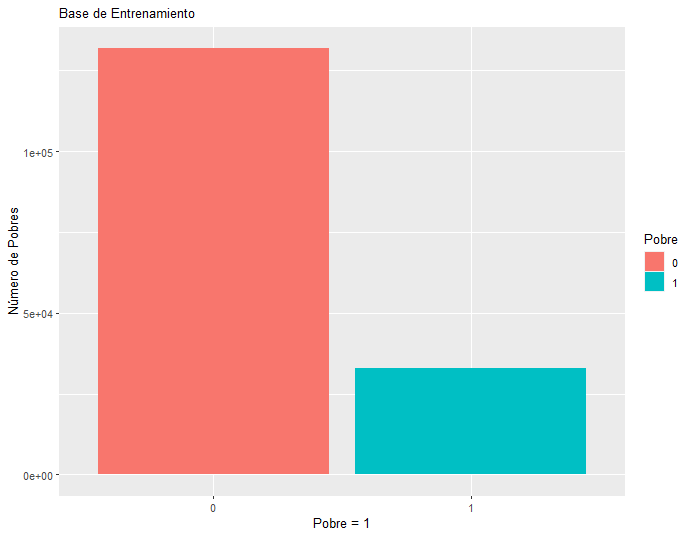
\includegraphics[width=\textwidth]{Graph 1 - Clases (Pobre y No Pobre).jpg}
\end{figure}

\begin{figure}[h]
\caption{Cajas y Bigotes Análisis de Ingreso - Colombia (2018)}
\centering
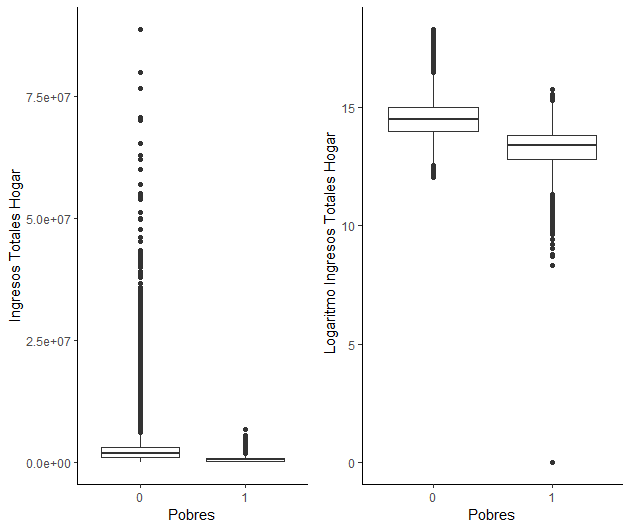
\includegraphics[width=\textwidth]{Graph 2 - Box-cox Ing vs. Pobre.jpg}
\end{figure}

\clearpage
\textbf{3. Anexos Modelos de Clasificación}
% Table created by stargazer v.5.2.3 by Marek Hlavac, Social Policy Institute. E-mail: marek.hlavac at gmail.com
% Date and time: dom., jul. 10, 2022 - 2:26:44 p. m.

\begin{table}[!htbp] \centering 
  \caption{Modelos iniciales} 
  \label{} 
  \scalebox{0.9}{\begin{tabular}{@{\extracolsep{5pt}}lccccc} 
\\[-1.8ex]\hline 
\hline \\[-1.8ex] 
 & \multicolumn{5}{c}{\textit{Dependent variable:}} \\ 
\cline{2-6} 
\\[-1.8ex] & \multicolumn{5}{c}{Pobre} \\ 
\\[-1.8ex] & (1) & (2) & (3) & (4) & (5)\\ 
\hline \\[-1.8ex] 
 Vivienda Propia =1 & $-$0.712$^{***}$ & $-$0.714$^{***}$ & $-$0.638$^{***}$ &  & $-$0.712$^{***}$ \\ 
  & (0.016) & (0.016) & (0.015) &  & (0.016) \\ 
  & & & & & \\ 
Número Total de Mujeres Hogar & 0.126$^{***}$ & 0.126$^{***}$ & 0.148$^{***}$ &  & 0.126$^{***}$ \\ 
  & (0.009) & (0.009) & (0.008) &  & (0.009) \\ 
  & & & & & \\ 
 Jefe de Hogar Mujer =1 & 0.038$^{**}$ & 0.040$^{***}$ &  & 0.142$^{***}$ & 0.038$^{**}$ \\ 
  & (0.015) & (0.015) &  & (0.013) & (0.015) \\ 
  & & & & & \\ 
Número de Ocupados Hogar & $-$0.715$^{***}$ & $-$0.715$^{***}$ & $-$0.782$^{***}$ &  & $-$0.715$^{***}$ \\ 
  & (0.011) & (0.011) & (0.009) &  & (0.011) \\ 
  & & & & & \\ 
 Edad Jefe Hogar & 0.002$^{***}$ & 0.002$^{***}$ &  & $-$0.023$^{***}$ & 0.001 \\ 
  & (0.001) & (0.001) &  & (0.0004) & (0.002) \\ 
  & & & & & \\ 
 Edad Jefe Hogar$^{2}$ &  &  &  &  & 0.00001 \\ 
  &  &  &  &  & (0.00002) \\ 
  & & & & & \\ 
 Núm. Menores Edad Hogar & 0.853$^{***}$ & 0.853$^{***}$ & 0.801$^{***}$ &  & 0.853$^{***}$ \\ 
  & (0.009) & (0.009) & (0.008) &  & (0.009) \\ 
  & & & & & \\ 
 Máx. Grado Escolar Jefe Hogar & $-$0.060$^{***}$ & $-$0.060$^{***}$ &  & $-$0.050$^{***}$ & $-$0.060$^{***}$ \\ 
  & (0.002) & (0.002) &  & (0.002) & (0.002) \\ 
  & & & & & \\ 
 Jefe Hogar Ocupado = 11 & $-$0.181$^{***}$ & $-$0.177$^{***}$ &  & $-$0.646$^{***}$ & $-$0.179$^{***}$ \\ 
  & (0.019) & (0.019) &  & (0.015) & (0.020) \\ 
  & & & & & \\ 
 Núm. Afiliados Salud Hogar & 0.061$^{***}$ & 0.062$^{***}$ & 0.092$^{***}$ &  & 0.062$^{***}$ \\ 
  & (0.007) & (0.007) & (0.007) &  & (0.007) \\ 
  & & & & & \\ 
 Uso Prod. Financieros Jefe Hogar = 1& $-$1.036$^{***}$ &  &  & $-$1.254$^{***}$ & $-$1.035$^{***}$ \\ 
  & (0.133) &  &  & (0.126) & (0.133) \\ 
  & & & & & \\ 
 Constante & $-$1.156$^{***}$ & $-$1.164$^{***}$ & $-$1.500$^{***}$ & 0.398$^{***}$ & $-$1.136$^{***}$ \\ 
  & (0.036) & (0.036) & (0.016) & (0.030) & (0.060) \\ 
  & & & & & \\ 
\hline \\[-1.8ex] 
Observations & 164,959 & 164,959 & 164,959 & 164,959 & 164,959 \\ 
Log Likelihood & $-$66,666.120 & $-$66,705.200 & $-$67,328.020 & $-$80,224.950 & $-$66,666.020 \\ 
Akaike Inf. Crit. & 133,354.200 & 133,430.400 & 134,668.000 & 160,461.900 & 133,356.000 \\ 
\hline 
\hline \\[-1.8ex] 
\textit{Note:}  & \multicolumn{5}{r}{$^{*}$p$<$0.1; $^{**}$p$<$0.05; $^{***}$p$<$0.01} \\ 
\end{tabular} }
\end{table}

%%% Grafica 3

\begin{figure}[h]
\caption{Comparación ROC de los modelos inciciales }
\centering
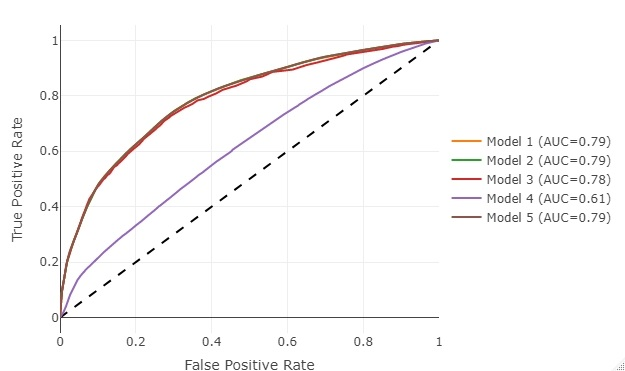
\includegraphics[width=120mm, scale=0.3]{Graph3 - Models ROC.jpg}
\end{figure}


% latex table generated in R 4.2.1 by xtable 1.8-4 package
% Sat Jul  9 21:11:07 2022
\begin{table}[ht]
\caption{Modelos estimados para mejorar capacidad predictiva} 
  \label{}
\centering
\begin{tabular}{rlrrrrrrrrrr}
  \hline
Model &  & lambda & ROC & Sens & Spec & Acc & Kappa \\ 
  \hline
Logit-Cross validation & 1 & none & 0.79 & 0.96 & 0.28 & 0.83 & 0.31  \\ 
Logit-Lasso Accuracy &  55 & 0154 & 0.79 & 0.97 & 0.23 & 0.83 & 0.28  \\ 
Logit-Lasso ROC & 54 & 0.01402 & 0.79 & 0.97 & 0.23 & 0.83 & 0.28  \\ 
Logit-Lasso Sensitivity & 100 & 1.02329 & 0.77 & 1.00 & 0.00 & 0.80 & 0.00 \\ 
Logit-Upsampling &  57 & 0.01855 & 0.79 & 0.75 & 0.69 & 0.72 & 0.43  \\ 
Logit-Downsampling &  57 & 0.01855 & 0.79 & 0.74 & 0.69 & 0.72 & 0.43 \\ 
   \hline
\end{tabular}
\end{table}

% latex table generated in R 4.2.1 by xtable 1.8-4 package
% Sat Jul  9 21:53:59 2022
\begin{table}[ht]
\centering
\caption{Alternate cutoff Closest topleftt ROC}
\begin{tabular}{rrrr}
  \hline
 & threshold & specificity & sensitivity \\ 
  \hline
1 & 0.53 & 0.73 & 0.71 \\ 
   \hline
\end{tabular}
\end{table}

\end{document}
